\chapter{EIGRP}

\section{Basic features}

Enhanced Interior Gateway Routing Protocol (EIGRP) is a powerful \emph{distance vector} routing protocol and is relatively easy to configure for basic networks. Features of EIGRP:

\begin{itemize}
\item Use DUAL algorithm
\item Use RTP  instead of TCP or UDP
\item Partial and Bounded Updates -- Sends updates only when there is a change and only to the routers that need the information
\item Supports Equal and Unequal cost load balancing
\item Does not encrypt the routing updates
\item Authentication: Only accepts routing information from other routers with the same authentication information 
\end{itemize}

\textbf{Protocol Dependent Modules (PDM)} sends and receives EIGRP packets that are encapsulated in IPv4 or IPv6. \textbf{Reliable Transport Protocol (RTP)} is responsible for both reliable and unreliable packet delivery, because EIGRP cannot use UDP or TCP. RTP can send EIGRP packets as unicast or multicast.

\section{Packet types}

\subsection{Hello packets}

EIGRP uses Hello packets to discover other EIGRP-enabled routers on directly connected links and form EIGRP neighbor adjacencies. These packets are sent as multicast \emph{every five seconds}. However, on slow network (e.g. multipoint, NBMA networks with access links of T1), they are sent as unicast packets every 60 seconds.\\
 
\textbf{Hold timer} determines the maximum time the router should wait to declare neighbor as unreachable. By default, the Hold timer is \emph{three times the Hello interval}. If the hold time expires, EIGRP declares the route as down and DUAL searches for a new path by sending out queries.\\

Hello intervals and hold times are configurable on a per-interface basis and \emph{do not have to match} with other EIGRP routers to establish or maintain adjacencies. If the Hello interval is changed, ensure that the Hold time value is not less than the Hello interval. Otherwise, neighbor adjacency goes down after the Hold timer expires and before the next Hello interval. 

\subsection{Other packets}

EIGRP sends \textbf{Update packets} to propagate routing information. These packets are sent only when necessary and to those routers that require it. This is known as \emph{bounded update}, which minimizes the network bandwidth. Update packets must also contain only the routing information needed, which is known as \emph{partial update}.\\

EIGRP sends \textbf{Acknowledgment packets} when RTP reliable delivery is used. An EIGRP acknowledgment is an EIGRP Hello packet without any data. RTP uses reliable delivery for Update, Query, and Reply packets.\\

DUAL uses \textbf{Query and Reply packets} when searching for networks and other tasks. Queries can use multicast or unicast, whereas replies are always sent as unicast.

\section{Encapsulating EIGRP Messages}

IP packet header, EIGRP packet header, and TLV (Type, Length, Value) field are encapsulated in a Layer 2 frame (Figure \ref{IPpacketHeader}). The destination MAC address of the frame is the multicast address \textbf{01-00-5E-00-00-0A}.\\

In the \textbf{IP packet header}, the protocol field is set to \textbf{88} to indicate EIGRP. The destination address is the multicast address \textbf{224.0.0.10} for IPv4, or \textbf{FF02::A} for IPv6. 

\begin{figure}[hbtp]
\caption{Encapsulating EIGRP Messages}\label{IPpacketHeader}
\centering
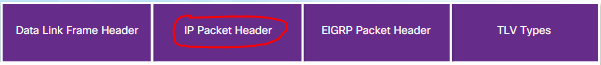
\includegraphics[ width=0.7\textwidth ]{pictures/IPpacketHeader.PNG}
\end{figure}

\begin{figure}[hbtp]
\centering
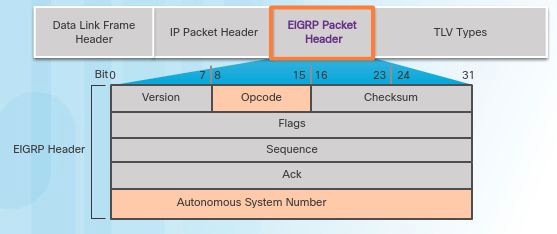
\includegraphics[width=0.6\textwidth]{pictures/EIGRP-packet-header.png}
\caption{EIGRP packet header} \label{EIGRP-packet-header}
\end{figure}

The \textbf{EIGRP packet header} contains two important fields: Opcode and Autonomous system number (Figure \ref{EIGRP-packet-header}). \textbf{Opcode field} specifies EIGRP packet type using number: Update(1), Query(3), Reply(4), and Hello(5). \textbf{Autonomous system (AS) number} specifies the EIGRP routing process. Unlike RIP, multiple instances of EIGRP can run on a network. The autonomous system number is used to track each running EIGRP instance.\\

There are three types of \textbf{TLV field}: EIGRP parameters (figure \ref{EIGRP-parameters}), IP internal routes (figure \ref{EIGRP-internal-route}), and IP external routes (figure \ref{EIGRP-external-route}).\\

\begin{figure}[hbtp]
\centering
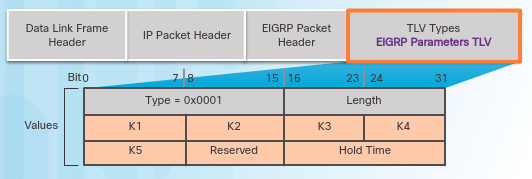
\includegraphics[width=0.6\textwidth]{pictures/EIGRP-parameters.png}
\caption{EIGRP TLV: EIGRP parameters} \label{EIGRP-parameters}
\end{figure}

The \emph{length} field identifies the size (in bytes) of the \emph{value} field. The \emph{value} field contains data for EIGRP message. The \emph{type} field specifies the type of TLV: EIGRP parameters (1), IP internal routes (258), and IP external routes (259).\\

\begin{figure}[hbtp]
\centering
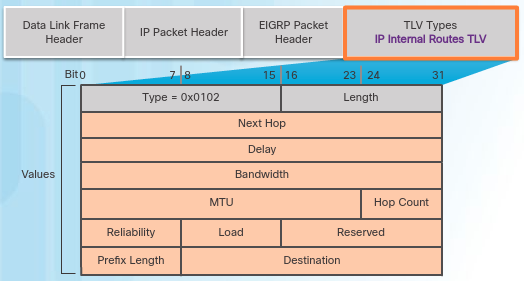
\includegraphics[width=0.6\textwidth]{pictures/EIGRP-internal-route.png}
\caption{EIGRP internal routes TLV fields} \label{EIGRP-internal-route}
\end{figure}

The \textbf{EIGRP parameters} include the weights that EIGRP uses for its composite metric (K1 -- K5). By default, only bandwidth and delay are weighted. Both are weighted equally; therefore, the K1 field for bandwidth and the K3 field for delay are both set to one (1). The other K values are set to zero (0).\\

\begin{figure}[hbtp]
\centering
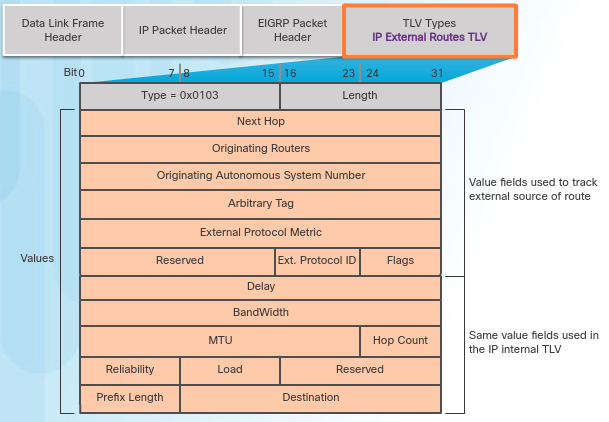
\includegraphics[width=0.6\textwidth]{pictures/EIGRP-external-route.png}
\caption{EIGRP external route TLV fields} \label{EIGRP-external-route}
\end{figure}
 
Each \textbf{IP internal route} or \textbf{IP external route} contains one route entry and the metric information for specific route. These types of TLV are included in EIGRP Update packets. The IP internal route message is used to advertise EIGRP routes within an autonomous system. The IP external message is used to import default static route, as well as routes outside the autonomous system, into the EIGRP routing process.
 
\section{Operation}

\subsection{Neighbor adjacency}
EIGRP uses Hello packets to establish and maintain neighbor adjacencies. To accomplish this, two EIGRP routers must use the same K values and autonomous system number.\\

\begin{figure}[hbtp]
\caption{Establish EIGRP adjacency}\label{EIGRPadjacency}
\centering
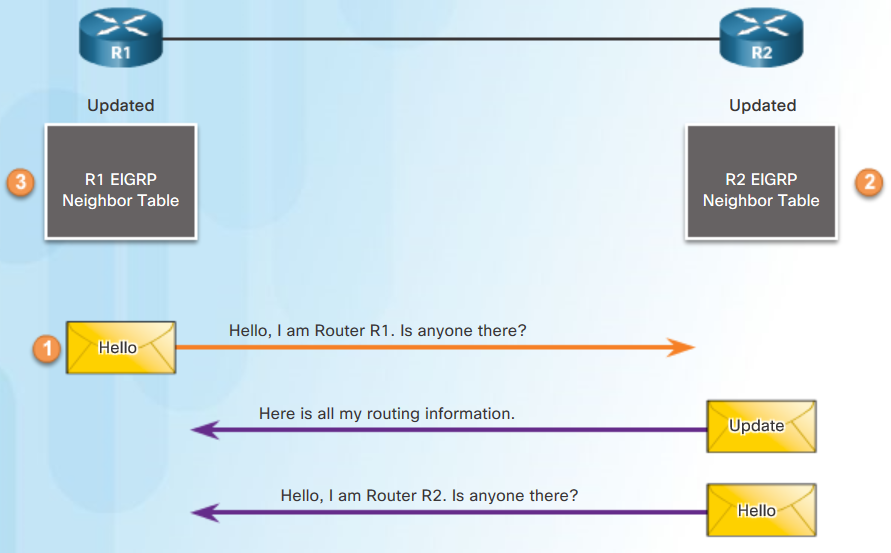
\includegraphics[ width=0.7\textwidth ]{pictures/EIGRPadjacency.PNG}
\end{figure}

 
Each EIGRP router maintains a neighbor table, which contains a list of routers that have an EIGRP adjacency with this router. The neighbor table is used to track the status of these EIGRP neighbors.\\

Figure \ref{EIGRPadjacency} shows two EIGRP routers exchanging initial EIGRP Hello packets. When an EIGRP enabled router receives a Hello packet on an interface, it adds that router to its neighbor table:

\begin{enumerate}
\item A new router (R1) comes up on the link and sends an EIGRP Hello packet through all of its EIGRP-configured interfaces.

\item Router R2 receives the Hello packet on an EIGRP-enabled interface. R2 replies with an EIGRP update packet that contains all the routes it has in its routing table, except those learned through that interface (split horizon). However, the neighbor adjacency is not established until R2 also sends an EIGRP Hello packet to R1.

\item After both routers have exchanged Hellos, the neighbor adjacency is established. R1 and R2 update their EIGRP neighbor tables adding the adjacent router as a neighbor.
\end{enumerate}

\subsection{Topology table}

The topology table includes all destinations advertised by neighboring (adjacent) routers and the cost (metric) to reach each network. When a router receives the EIGRP update from a neighbor, it adds all update entries to its topology table. Because EIGRP update packets use RTP reliable delivery, the router replies with an EIGRP acknowledgment packet.

\subsection{Metric}

By default, EIGRP uses the following values in its composite metric to calculate the preferred path to a network:

\begin{itemize}
\item \textbf{Bandwidth} -- The slowest bandwidth among all of the outgoing interfaces, along the path from source to destination.
\item \textbf{Delay} -- The cumulative (sum) of all interface delay along the path (in tens of microseconds).
\end{itemize}

Default composite formula:
\[ \text{metric} = \left( \text{bandwidth} + \text{delay} \right) \times 256 \]

Complete composite formula:
\[ \text{metric} = \left( K1\times\text{bandwidth} + \frac{K2\times\text{bandwidth}}{256 - \text{load}} + K3\times\text{delay} \right) \times \frac{K5}{K4+\text{reliability}}\]
This is a conditional formula. If $K5=0$, the last term is replaced by 1. Default values for each parameter:

\begin{itemize}
\item K1 (bandwidth) = 1
\item K2 (load) = 0
\item K3 (delay) = 1
\item K4 (reliability) = 0
\item K5 (reliability) = 0
\end{itemize}

\paragraph{Examining interface metric values:} The \verb|show interfaces <interface>| command displays interface information (figure \ref{EIGRPmetric}), including the parameters used to compute the EIGRP metric.

\begin{figure}[hbtp]
\caption{Examine interface metric values}\label{EIGRPmetric}
\centering
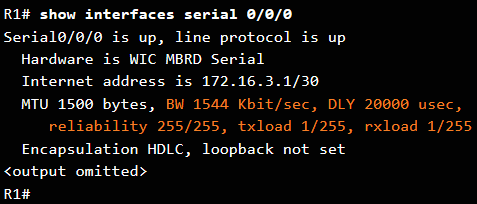
\includegraphics[scale=0.8]{pictures/EIGRPmetric.PNG}
\end{figure}

\begin{itemize}
\item \textbf{BW} -- Bandwidth of the interface (in kilobits per second).
\item \textbf{DLY} -- Delay of the interface (in microseconds).
\item \textbf{Reliability} - Reliability of the interface as a fraction of 255 (255/255 is 100\% reliability), calculated as an exponential average over five minutes. By default, EIGRP does not include its value in computing its metric.
\item \textbf{Txload, Rxload} -- Transmit and receive load on the interface as a fraction of 255 (255/255 is completely saturated), calculated as an exponential average over five minutes. By default, EIGRP does not include its value in computing its metric.
\end{itemize}

\paragraph{Bandwidth:} EIGRP uses the slowest bandwidth along the path to the destination network. EIGRP divides a reference bandwidth value of $10^7$ by the interface bandwidth value in kb/s. If the result is not a whole number, then the value is rounded down. For example, $10^7$ divided by 1024 equals 9765.625. The .625 is dropped to yield 9765 for the bandwidth portion of the composite metric.

\paragraph{Delay:} EIGRP uses the sum of all delays along the path to the destination. The sum of these delays is divided by 10. See also table \ref{delay-value} for default delay values. For example, along the path R1$\rightarrow$R2$\rightarrow$R3, the s0/0/1 interface on R2 has a delay of 20,000 microseconds, the g0/0 interface on R3 has a delay of 10 microseconds. The delay is $ \left( 20000 + 10 \right) \div 10 = 2001 $.

\begin{table}[h!]
\centering
\caption{Default delay values}
\label{delay-value}
\begin{tabular}{|l|l|}
\hline
Media            & Delay \\ \hline
Ehternet         & 1000  \\ \hline
Fast Ethernet    & 100   \\ \hline
Gigabit Ethernet & 10    \\ \hline
Serial link      & 20000 \\ \hline
\end{tabular}
\end{table}

\subsection{DUAL algorithm}

EIGRP uses the Diffusing Update Algorithm (DUAL) to provide the best loop-free path and loop-free backup paths. DUAL uses several terms, which are discussed in more detail throughout this section:

\begin{itemize}
\item \textbf{Successor} is a neighboring router that is used for packet forwarding and is the least-metric route to the destination network. The IP address of a successor is shown in a routing table entry right after the word via (see figure \ref{EIGRP-FD}). 

\item \textbf{Feasible Distance (FD)} is the metric of the Successor to reach the destination network. FD is listed in the routing table entry as the second number inside the brackets (see figure \ref{EIGRP-FD}).

\item \textbf{Feasible Successor (FS)} is a neighbor that has a loop-free backup path to the same network as the successor, and it satisfies the Feasibility Condition (FC). FS is not represented in the routing table until the Successor is down. Instead, we can view FS in topology table (figure \ref{FS}).

\item \textbf{Reported Distance (RD)} is the FD (metric) of an FS to the same destination network.

\item \textbf{Feasible Condition (FC)} is met when a neighbor's RD to a network is less than the local router's FD to the same one. If the RD is less, it represents a loop-free path. 
\end{itemize}

\begin{figure}[hbtp]
\centering
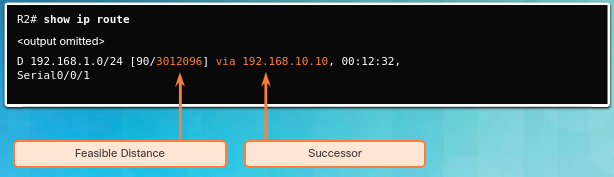
\includegraphics[ width=0.8\textwidth ]{pictures/EIGRP-FD.png}
\caption{Successor and Feasible Distance} \label{EIGRP-FD}
\end{figure}

A route learned through EIGRP must meet two criteria to be installed in the local routing table:

\begin{itemize}
\item The route must be loop-free, being either an FS or having an RD that is less than the total distance.

\item The metric of the route must be lower than the metric of the best route (the successor) multiplied by the \emph{variance} configured on the router. For example, if the variance is set to 1, only routes with the same metric as the successor are installed in the local routing table. If the variance is set to 2, any EIGRP-learned route with a metric less than 2 times the successor metric will be installed in the local routing table.
\end{itemize}

The decision process for all route computations is done by the DUAL Finite State Machine (FSM). The DUAL FSM tracks all routes and uses EIGRP metrics to select efficient, loop-free paths, and to identify the routes with the least-cost path to be inserted into the routing table.\\

\begin{figure}[hbtp]
\caption{Feasible Successor in Topology table}\label{FS}
\centering
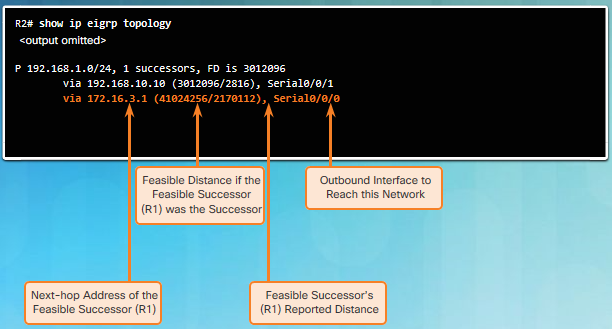
\includegraphics[ width=0.8\textwidth ]{pictures/FS.PNG}
\end{figure}


Recomputation of the DUAL algorithm can be processor-intensive. EIGRP avoids recomputation whenever possible by maintaining a list of backup routes that DUAL has already determined to be loop-free. If the primary route in the routing table fails, the best backup route is immediately added to the routing table.\\

\begin{figure}[hbtp]
\centering
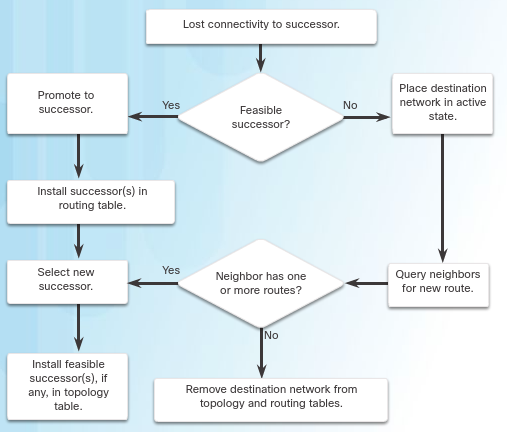
\includegraphics[width=0.7\textwidth]{pictures/EIGRP-DUAL.png}
\caption{DUAL Finite State machine} \label{EIGRP-DUAL}
\end{figure}

When the Successor is no longer available and there is no FS, DUAL puts the route into an \emph{active} state. DUAL sends EIGRP queries asking other routers for a path to the network. Other routers return EIGRP replies, letting the sender of the EIGRP query know whether or not they have a path to the requested network. If none of the EIGRP replies have a path to this network, the sender of the query does not have a route to this network. See also figure \ref{EIGRP-DUAL}.

\subsection{Automatic summarization}

Route summarization allows a router to group networks together and advertises them as one large group using a single, summarized route. Summarization decreases the number of entries in routing updates and lowers the number of entries in local routing tables. It also reduces bandwidth utilization for routing updates and results in faster routing table lookups. However, in classes IP network, the only way that all routers can find the best routes for each individual subnet is for neighbors to send subnet information. In this situation, automatic summarization should be disabled. \\

A problem associated with automatic summarization is that a summary address also advertises networks that are not available on the advertising router. For example, R1 is advertising the summary address 172.16.0.0/16, but it is only connected to 172.16.1.0/24. Therefore, R1 may receive incoming packets to destinations that do not exist (for example, 172.16.2.0/24). It then forwards a request to a destination network that does not exist, creating a routing loop.\\

EIGRP uses the Null0 interface to avoid the above problem. The Null0 interface is a virtual IOS interface that is a route to nowhere. If R1 receives a packet destined for a network that is advertised by the classful mask but does not exist, it discards the packets by sending them to Null0.\\
 
\note The Null0 summary route is removed when automatic summarization is disabled.\\
\note EIGRP for IPv4 automatic summarization is disabled by default.

\section{Configuration}

\subsection{EIGRP for IPv4}

\begin{enumerate}
\item Enable EIGRP routing with AS number
	\begin{verbatim}
	R1(config)# router eigrp 10
	\end{verbatim}
	
\item (Optional) Disable auto summarization using \verb|no auto-summary| command.
	
\item Advertise the directly connected networks using the wildcard mask
	\begin{verbatim}
	R1(config-router)# do show ip route | inc C
	R1(config-router)# network 10.1.1.0 0.0.0.3
	R1(config-router)# network 192.168.1.0 0.0.0.255 
	R1(config-router)# network 10.3.3.0 0.0.0.3
	\end{verbatim}
	
\item Configure passive interfaces 
	\begin{verbatim}
	R1(config-router)# passive-interface g0/0
	R1(config-router)# passive-interface g0/1
	\end{verbatim}
	
\item If there are too many passive interfaces, you can make all interfaces of the router to be passive using \verb|passive-interface default|, then configure necessary interface to be active again using \verb|no passive-interface|
	\begin{verbatim}
	R1(config-router)# passive-interface default
	R1(config-router)# no passive-interface s0/0/0
	R1(config-router)# no passive-interface s0/0/1
	\end{verbatim}
	
\item On border router, propagate its default static route to other routers
    \begin{verbatim}
    R1(config-router)# redistribute static
    \end{verbatim}

\item Examine the EIGRP neighbor table (figure \ref{neigborTable}), routing table using \verb|show ip route eigrp| (figure \ref{EIGRProutingTable}), topology table using \verb|show ip eigrp topology| (figure \ref{EIGRPtopologyTable}), EIGRP routing parameters, passive interfaces and networks advertised (figure \ref{EIGRPparameters}).
	\begin{figure}[hbtp]
	\caption{Examine EIGRP neigbor table}\label{neigborTable}
	\centering
	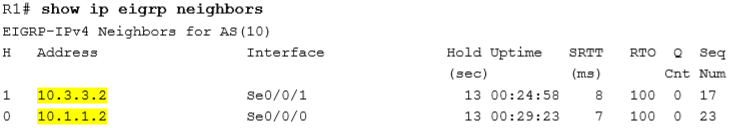
\includegraphics[scale=0.8]{pictures/neigborTable.PNG}
	\end{figure}
	
	\begin{figure}[hbtp]
		\caption{EIGRP routing table}\label{EIGRProutingTable}
		\centering
		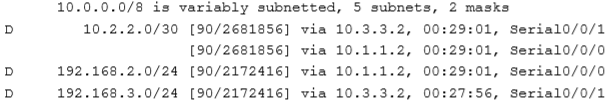
\includegraphics[scale=0.8]{pictures/EIGRProutingTable.PNG}
		\end{figure}
 	
	\begin{figure}[hbtp]
			\caption{EIGRP topology table}\label{EIGRPtopologyTable}
			\centering
			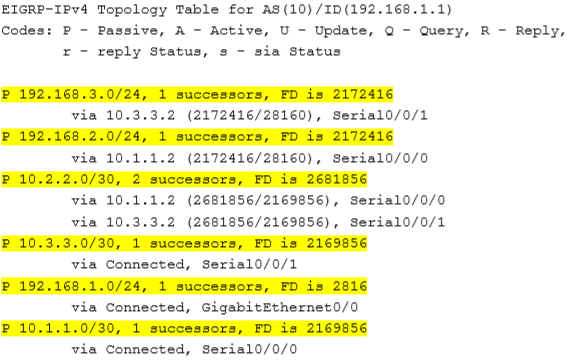
\includegraphics[scale=0.8]{pictures/EIGRPtopologyTable.PNG}
			\end{figure}


	\begin{figure}[hbtp]
	\caption{EIGRP routing parameters and networks advertised}\label{EIGRPparameters}
	\centering
	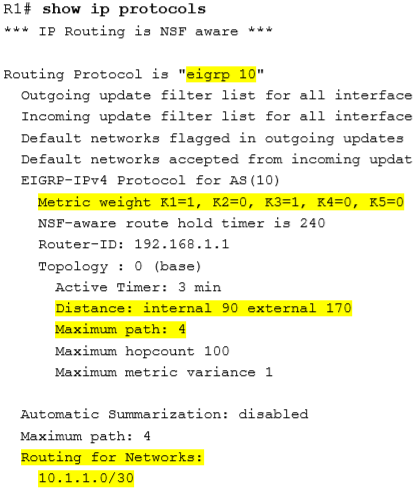
\includegraphics[scale=0.8]{pictures/EIGRPparameters.PNG}
	\end{figure}
						
\end{enumerate}

\subsection{EIGRP for IPv6}

\begin{enumerate}
\item Enable IPv6 routing on the router
	\begin{verbatim}
	R1(config)# ipv6 unicast-routing 
	\end{verbatim}
	
\item Enable EIGRP for IPv6
	\begin{verbatim}
	R1(config)# ipv6 router eigrp 1 
	R1(config-router)# no shutdown 
	\end{verbatim}	
	
\item Assign a router ID to each router and 
	\begin{verbatim}
	R1(config)# ipv6 router eigrp 1 
	R1(config-router)# eigrp router-id 1.1.1.1
	\end{verbatim}

\item Configure passive interfaces
	\begin{verbatim}
	R1(config)# ipv6 router eigrp 1 
	R1(config-router)# passive-interface g0/0 
	\end{verbatim}
	
\item If there are too many passive interfaces, you can make all interfaces of the router to be passive using \verb|passive-interface default|, then configure necessary interface to be active again using \verb|no passive-interface|
	\begin{verbatim}
	R1(config-router)# passive-interface default
	R1(config-router)# no passive-interface s0/0/0
	R1(config-router)# no passive-interface s0/0/1
	\end{verbatim}	
	
\item Configure EIGRP for IPv6 with AS number on each interface
	\begin{verbatim}
	R1(config)# interface g0/0 
	R1(config-if)# ipv6 eigrp 1 
	R1(config-if)# no shutdown
	\end{verbatim}
	
\item On border router, propagate its default static route to other routers
    \begin{verbatim}
    R1(config-router)# redistribute static
    \end{verbatim}
	
\item Examine the neighbor adjacencies using \verb|show ipv6 eigrp neighbors|, routing table using \verb|show ipv6 route eigrp|, topology table using \verb|show ipv6 eigrp topology|. Verify the parameters and current state of the EIGRPv6 using \verb|show ipv6 protocols|.
	
\end{enumerate}

\subsection{Tuning EIGRP}

\paragraph{Bandwidth utilization:} By default, EIGRP uses only up to \textbf{50\%} of an interface's bandwidth for EIGRP information. This prevents the EIGRP process from over-utilizing a link and not allowing enough bandwidth for the routing of normal traffic. Use the following command to configure the 80\% of bandwidth that can be used by EIGRP (AS = 100) on an interface.

\begin{verbatim}
Router(config-if)# ip bandwidth-percent eigrp 100 80
Router(config-if)# ipv6 bandwidth-percent eigrp 100 80
\end{verbatim}

\paragraph{Hello and Hold timers:} Hello intervals and hold times are configurable on a per-interface basis and do not have to match with other EIGRP routers to establish or maintain adjacencies. If the Hello interval is changed, ensure that the hold time value is equal to, or greater than, the Hello interval. The following commands set Hello interval to 50 seconds and Hold timer to 150 seconds. The number \verb|100| is the AS number of EIGRP. \note The \emph{seconds} value for both Hello and Hold time intervals can range from 1 to 65,535. 

\begin{verbatim}
Router(config-if)# ip hello-interval eigrp 100 50
Router(config-if)# ip hold-time eigrp 100 150
\end{verbatim}

\paragraph{Equal-cost load balancing:} Load balancing is the ability of a router to distribute outbound traffic using all interfaces that have the same metric from the destination address. For IP, Cisco IOS Software applies load balancing using up to \emph{four} equal-cost paths by default. However, this can be modified using the below command. If the \verb|<value>| is set to 1, load balancing is disabled.  The \verb|show ip protocols| command can be used to verify the number of equal-cost paths currently configured on the router.

\begin{verbatim}
Router(config-router)# maximum-paths <value>
\end{verbatim} 

\paragraph{Unequal-cost load balancing:} EIGRP is the only routing protocol that supports unequal-cost load balancing. Setting a variance value using the following command enables EIGRP to install routes with unequal cost in a local routing table. 

\begin{verbatim}
R1(config-router)# variance 2
\end{verbatim}

